% !TeX program = xelatex
\documentclass[3pt,landscape]{article}
\usepackage{multicol, calc, ifthen, amsmath, amsthm, amsfonts, amssymb, color, graphicx, hyperref, fontspec, xunicode}

\usepackage[landscape]{geometry}

\defaultfontfeatures{Mapping=tex-text,Scale=MatchLowercase}
\ifthenelse{\lengthtest { \paperwidth = 11in}}
    { \geometry{top=.3in,left=.3in,right=.3in,bottom=.3in} }
    {\ifthenelse{ \lengthtest{ \paperwidth = 297mm}}
        {\geometry{top=1cm,left=1cm,right=1cm,bottom=1cm} }
        {\geometry{top=1cm,left=1cm,right=1cm,bottom=1cm} }
    }
\pagestyle{empty}
\makeatletter
\setmainfont{Source Sans Pro}
\setmonofont{Menlo}
\DeclareMathSizes{3}{3}{2}{1}

\renewcommand{\section}{\@startsection{section}{1}{0mm}{-1ex plus -.5ex minus -.2ex}{0.5ex plus .2ex}{\normalfont\large\bfseries}}
\renewcommand{\subsection}{\@startsection{subsection}{2}{0mm}{-1explus -.5ex minus -.2ex}{0.5ex plus .2ex}{\normalfont\normalsize\bfseries}}
\renewcommand{\subsubsection}{\@startsection{subsubsection}{3}{0mm}{-1ex plus -.5ex minus -.2ex}{1ex plus .2ex}{\normalfont\small\bfseries}}
\makeatother
\setcounter{secnumdepth}{0}
\setlength{\parindent}{0pt}
\setlength{\parskip}{0pt plus 0.5ex}
\hypersetup{colorlinks=true, urlcolor=blue}
\def\ci{\perp\!\!\!\perp}

%%%%%%%%%%%%%%%%%%%%%%%%%%%%%%%%%%%%%%%%%%%%%%%%%%

\begin{document}
\raggedright
\footnotesize

\begin{multicols}{3}
\setlength{\premulticols}{1pt}
\setlength{\postmulticols}{1pt}
\setlength{\multicolsep}{1pt}
\setlength{\columnsep}{2pt}

\begin{center}
    \Large{\underline{Data Science Mini Field Guide}} \\
\end{center}
% \begin{center}
%     Written by: \href{http://krishna.im}{Krishna Parashar}\\
%     Published by: \href{http://www.atrus.co}{Atrus}\\
% \end{center}

%%%%%%%%%%%%%%%%%%%%%%%%%

\section*{Introduction}

Data Science: Hacking Skill \& Math \& Statistics \& Expertise
Research: Math \& Statistics \& Expertise
Machine Learning: Hacking Skill \& Math \& Statistics

\textbf{Database Engineer}
\begin{itemize}
\item Experience with No-SQL systems: SQL systems, i.e. column-family stores, text and XML DBs,
\item Data cleaning: resolving entities, fuzzy matching, bounds checking etc.
\item Schema-on-read (or never) – late-commitment semantics of data
\item Data validation, using checksums, range checks statistical checks.
\end{itemize}


\textbf{Scientific Computing Expert }
\begin{itemize}
\item We were looking for the recent trend in scientific computing toward integration of machine learning as an adjunct or alternative to precise physical modeling (examples in lecture and one of the project topics). So skill in modeling with ML is important. 
\item Another answer was skill in using cluster tools (Spark, Hadoop, GraphLab etc.). 
\end{itemize}


\textbf{Machine Learning Expert}
\begin{itemize}
\item Appropriateness of particular algorithms for various types of data
\item Also how to featurize data, BOW, n-grams, skip-grams, dependency parsing.
\item Knowledge of ML toolkits: tuning for performance and accuracy 
\end{itemize}


\textbf{Jeff Hammerbacher’s Model}
\begin{itemize}
\item Identify problem
\item Instrument data sources
\item Collect data
\item Prepare data
\item Build model
\item Evaluate model
\item Communicate results
\end{itemize}


\section*{Data Collection}

CS 194 - Midterm Notes
\# Lecture 1: Introduction

Data Science: Hacking Skill + Math \& Statistics + Expertise
Research: Math \& Statistics + Expertise
Machine Learning: Hacking Skill + Math \& Statistics


Database Engineer
- Experience with No-SQL systems: SQL systems, i.e. column-family stores, text and XML DBs,
- Data cleaning: resolving entities, fuzzy matching, bounds checking etc.
- Schema-on-read (or never) – late-commitment semantics of data
- Data validation, using checksums, range checks statistical checks.

Scientific Computing Expert 
- We were looking for the recent trend in scientific computing toward integration of machine learning as an adjunct or alternative to precise physical modeling (examples in lecture and one of the project topics). So skill in modeling with ML is important. 
- Another answer was skill in using cluster tools (Spark, Hadoop, GraphLab etc.). 

Machine Learning Expert
- Appropriateness of particular algorithms for various types of data
- Also how to featurize data, BOW, n-grams, skip-grams, dependency parsing.
- Knowledge of ML toolkits: tuning for performance and accuracy 

Jeff Hammerbacher’s Model
1. Identify problem
2. Instrument data sources
3. Collect data
4. Prepare data
5. Build model
6. Evaluate model
7. Communicate results

What’s hard about Data Science?
1. Overcoming assumptions
2. Making ad-hoc explanations of data patterns
3. Overgeneralizing
4. Communication
5. Not verifying enough (model validation, data pipeline integrity, etc.)

\# Lecture 2: Data Preparation

ETL: Extract, Transform, Load
1. Extract data from the source
2. Load data into the sink
3. Transform data at source into a staging area

Some examples of sinks are: Python, R, SQLite, NoSQL stores
Source can be anything, from structured to unstructured data

Schema

Schema specify the structure and types of a data repository, and specify constraints within or between data fields. They are traditionally schema-on-write, and you can’t write data into a table without a schema.

However, new data stores are schema-on-read or schemaless.

    CREATE SCHEMA Sprockets
    CREATE TABLE NineProngs (source int, cost int, partnumber int) GO
    INSERT INTO NineProngs (source, cost, partnumber) VALUES (5, 100, 45312453)

 XML
- Generalizes HTML and helps to encode data, e.g. DOM.
- Data can be represented and stored without schema
- More verbose (not true after compression or in DB)
- Standard query/transformation languages like XSLT and Xquery
- Use Mark Logic Server as tooling
- Example of defining an XML Schema to the right. 
 

 JSON
- Schemaless data description language. 
- Typically used to represent hierarchical data structures. Procedural in the target language.
- More succinct in ASCII form.
- Transformation/ingestion rely on code.
- Use MongoDB as modeling

Tabular Data
- Table is a collection of rows and columns
- Each row has an index, and each column has a name
- Cell is specified by an (index, name) pair
- Cell may or may not have a value
- Schema = minimally column types
- Can be stored as CSV or TSV

Syslog – A standard for System Messages (Splunking)
- Grab data from many machines
- Check for unusual events: disk problems, network congestion, security attacks
- Monitor resources: network, memory usage, disk use, latency, threadss
- Dashboard for cloud administration

Event-Driven Parsing: SAX
Finds all the open-close tag events in XML documents and does callbacks to user code.
- User code can respond to subset of events it’s interested in
- User code can correctly compute aggregates from the data instead of implementing for each tag
- User code has to implement statement to keep track of where it is in the DOM tree
- User code can implement recover strategies for ill-formed XML
- Jackson and JSON-simple work the same for JSON.

Web Services
A web service is a software system designed to support interoperable machine to machine interaction over a network. There are two kinds of interactions: XML-based (SOAP), or RESTful interactions.

SOAP: Simple Object Access Protocol
SOAP RPC messages typically encode arguments that are presented to calling program as parameters and return values. This is longer because it requires a request-response cycle and often longer conversations. Both endpoints need to agree on the state. Design emphasis is on verbs, e.g. getUser(), addUser().

REST: Representation State Transfer
Stateless Client/Server Protocol. Each message in the protocol contains all the information needed by the receiver to understand or process it. Keeps things simple, with a set of well-defined list of operations (POST, GET, …). Resources are typically stored in a structured data format that supports hypermedia links, such as XHTML or XML. Design emphasis is on nouns, e.g. user location.

Data Cleaning
OpenRefine is a spreadsheet-like tool checking data quality and reformats, substitutes, constraint checks, etc.

Data Exploration
Histograms can show:
- Skewed distributions, long-tailed data
  - To deal with long-tailed data, you can sort histogram counts by descending magnitude, and plot count vs bucket number on a log-log plot.

  - Characteristic of social-influence processes
  - Also called preferential attachment models.
- Multimodal data
  - Arise from gender/political views, other binary factors
  - Explore further by using a color and histogram of multiple populations
- Weird data
  - Compare with previous pictures of OK data

Scatter plots can quickly expose relationships between two variables.

For multiple variables, we can use:
1. Stacked Plots, where stack variable is discrete.

2. Parallel Coordinate Plot: One discrete variable, and an arbitrary number of other variables.

3. Radar Chart: One discrete variable with an arbitrary number of other variables.

Principal Component Analysis
Allows visualization of high-dimensional continuous data in 2D using principal components, and will from the orthogonal dimensions in the dataset. Great for Dimensionality Reduction.

Conclusion
Beware of Martian Canals (false conclusions) - expect the unexpected!

\# Lecture 3: Manipulating Tabular Data

Structured Data
Data model is a collection of concepts for describing data.
Schema is a description of a particular collection of data.

Relational database is a set of relations (true for certain arguments).
A relation is made of 2 parts:
- Schema: specifies name of relation, plus name and type of each column
- Instance: the actual data at a given time. 

SQL is a Data Definition Language and Data Manipulation Language. 

SQL Calls

Creating Tables
`CREATE TABLE Students (sid CHAR(20), name CHAR(20), login CHAR(10), age INTEGER, gpa FLOAT)`

Adding and Deleting Tuples
`INSERT INTO Students (sid, name, login, age, gpa) VALUES ('53688', 'Smith', 'smith@ee', 18, 3.2)`

Basic SQL Query
Select target-list from relation-list where qualification

Joins and Inferences
`SELECT S.name, M.mortality FROM Students S, Mortality M WHERE S.Race=M.Race`

Inner Joins
`SELECT S.name, E.classid FROM Students S (INNER) JOIN Enrolled E ON S.sid=E.sid `

For unmatched keys on both sides, they are not input into the final table.

Left Outer Join and Right Outer Join – the unmatched on the left and right respectively get put into the final table. Full Outer Join – unmatched on both sides get put into the final table.

Left Semi Join – only return the rows on the left if there’s a match on both tables.

Cross Join – combines all possibilities from both tables

Theta Join – allows for arbitrary comparison relationships.

Conceptual strategy when evaluating SQL calls:
- Do FROM clause (cross-product), WHERE clause (conditions), SELECT clause (projection), DISTINCT clause (duplicate elimination)

Normalization

Process of minimizing data redundancy. Includes a foreign key to the information in another table for repeated data. The original table is the result of inner joins between tables.

SQLite
Table has fixed number of named columns of specified type.

5 storage classes for columns:
- Null
- Integer
- Real
- Text
- Blob

Reductions and Group By

Use GroupBy to select which columns to average, count, sum, average, min, max.

    SELECT SID, Name, AVG(GPA)
     FROM Students
     GROUP BY SID
 

Pandas / Python

- Positives: Pandas is lightweight and fast, full SQL expressiveness plus expressiveness of Python, integration with plotting functions like Matplotlib.
- Negatives: Tables must fit into memory. No post-load indexing functionality, indices are built when a table is created. No transactions or journalings. Large and complex joins are slow.

Series
- Keys of dictionary are indexes, built on NumPy’s `ndarray`

DataFrame
- Tables with named columns represented as a dictionary
- Each Series object represents a column

Operations
- Map, filter, sort, group by, aggregate, pivot or reshape
- Relational functions, e.g. union, joins, renames

Online Analytical Processing - OLAP

- Like a n-dimensional spreadsheet (cube)
- Columns become dimensions, where some of the variables are used as qualifiers, whereas those that we want to measure are normally numeric


Aggregation
- We can project a field on another axis, and then this is precomputed and maintained automatically in an OLAP cube, so queries are instantaneous. This helps to support real-time querying.
- However, aggregates increase space and cost of updates, but storage overhead is still small
- Good integration with clients
- Numpy and Matlab use dense nd-arrays which are OLAP


What’s Wrong with RDBMS Tables?
- Indices: Typical RDBMS tables mostly use indices, but we can’t afford this for large datastores
- Transactions: Safe state changes require journals and are slow
- Relations: Checking relations adds further overhead to updates
- Sparse Data Support: Very wasteful, however there is both row-based and column-based

NoSQL Storage Systems
- Cassandra, CouchDB (JSON), Pig (sequences of MapReduce Jobs), Hive (relational database built on Hadoop, developed at Facebook)
- Could be dynamic columns, or no schema (like CouchDB)

Pig 

- SQL functionality built on top of Hadoop
- Example Problem

 
\# Lecture 4: Statistics
Measurements
- Properties like min, max, mean, std. dev.
- Relationships: scatter plots, regression, correlation
- For models: accuracy, performance

A Null hypothesis is essentially the position a devil’s advocate would take when evaluating the results of an experiment (there is no difference in data samples or that difference is a certain value).
The p-value is the probability of a statistic value at least as extreme as the observation given that the null hypothesis is true.
- High p-value your data are likely with a true null.
- Low p-value: your data are unlikely with a true null.

Samples
- We usually only have samples from an infinite population
- Sample measurements have variance, and bias.
- Unbiased includes sample mean and median. Biased includes min and max. Variance:

Variance 
Central Limit Theorem
- The distribution of the sum of a set of n identically-distributed random variables $X_i$ approaches a normal distribution as n goes to infinity
- Many statistical tools including mean and variance, t-test, ANOVA assume data are normally distributed

Distributions
- Normal -- Bell Curve -- often assume for stats
- Bi/Multinomial -- \# events of N tries
Heavily skewed:
- Poisson -- \# events given fixed rate
- Exponential -- time between fixed rate events
- “Power law” -- line on log-log -- word freq

- Poisson: distribution of counts that occur at a certain rate, e.g. web site clicks
- Exponential: Interval between two such events
- Zipf/Pareto/Yule: Govern the frequencies of different terms in a document, or web site visits
- Binomial / Multinomial: The number of counts of events (e.g. die tosses) out of n trials

Rhine Paradox: Experiment where the act of telling psychics that they have psychic abilities causes them to lose it

Hypothesis Testing:
- A test statistic is some measurement we can make on the data which is likely to be big under the hypothesis we want to prove ($H_A$) but small under the null hypothesis ($H_O$).
- E.g. we are trying to prove a biased coin. We set the test statistic to be that the coin flips heads many times. 
  - $H_A$ = Coin is biased
  - $$H_0$$ = Coin is fair (to be disproved!)
- Instead of proving the hypothesis, we attempt to disprove the null hypothesis ($$H_0$$)
- One-tailed or two-tailed. Two-tailed test is convenient because it checks either very large or very small counts of heads.
- $$H_0$$: null hypothesis that mean(A) = mean(B). We Reject if Pr(x > s | $$H_0$$) < p is small, e.g. less than 0.05.

Types of Error


Three Important Tests
- T-test: compare two groups to see if they have the same distribution
  - test statistic -  t = sample mean / sample s.d.
  - This is known as the t-distribution
  - You could also have a single-sample test for one group of individuals in two conditions.
  - This is called a within-subjects design
- Chi-squared and Fisher’s test: Compare counts in a contingency table
  - Test whether an observation is consistent with the data
  - 

  - Fisher’s exact test works when counts are under different conditions
- ANOVA (ANalysis Of VAriance) 
  - Compare outcomes under several discrete interventions
- All the above tests are parametric: 
  - Assume the data are 
    - normally distributed
    - the samples are independent of each other and all have the same distribution (IID). 
- Non-parametric tests (assume nothing about distribution)
  - K-S test
    - useful test for checking whether two (continuous or discrete) distributions are the same. 
      - Such as testing if a distribution is normal
      - Or testing to make sure your data is similar to data produced by your pipeline. 
    - one-sided test is compared against a reference distribution
    - two observed distributions are compared
    - K-S statistic is just the max distance between the CDFs of the two distribution
  - Permutation Tests
  - Bootstrap sampling
    - Sampling your sample
    - Boostrap Confidence Interval tests to see if the 95% CI contains what we predict.

Train Test Validation
- Split data into training, test and validation sets
  - Validation set is used for parameter tuning
  - 60–20-20 split

Feature Selection
- Method 1: Ablation
  - Train a model on features ($f_1,…, f_n$), measure performance $Q_0$ 
  - Remove a feature and remeasure performance. 
  - If new performance is significantly (by some t-test) worst than $Q_0$, then don’t remove the feature. 
- Method 2: Mutual Information
  - Mutual information measures the extent to which knowledge of one feature influences the distribution of another (the classifier output).
- Method 3: Chi-Squared Test 
  - CHI-squared is an important statistic to know for comparing count data.  
- Feature Hashing 
  - Allows us to make sense of very rare features (such as URLs) by hashing them into similar categories and just keeping a count of features that fill a hash. 
  

\# Lecture 5: NLP
Basic Terms: 
- Syntax: the allowable structures in the language: sentences, phrases, affixes (-ing, -ed, -ment, etc.).
- Semantics: the meaning(s) of texts in the language.
-  Part-of-Speech (POS): the category of a word (noun, verb, preposition etc.).
- Bag-of-words (BoW): a featurization that uses a vector of word counts (or binary) ignoring order.
- N-gram: for a fixed, small N (2-5 is common), an n-gram is a consecutive sequence of words in a text. 
Bag of Words Featurization 
- Map words to a unique integer and store as a sparse vector (id, count):
  - (1,2),(3,1),(5,1),(12,1),(14,1) 
- original word order is lost, replaced by the order of id’s.
  - common to discard infrequent words 
  - follow power law distribution 
- tf-idf weighting
  - tf- term frequency - within the document 
  - idf - inverse domain frequency  - more rare words weighted more
  - tf-idf weighting can make BoW featurization more powerful
- Use cosine distance with some sort of weightings to optimize Bag of Words
  
N-grams
- modeling tuples of consecutive words
  - Sentence:  The        cat      sat      on        the          mat 
  - 3-grams: the-cat-sat, cat-sat-on, sat-on-the, on-the-mat 
- Using n-grams+BoW improves accuracy over BoW alone for classifying and other text problems. A typical performance (e.g. classifier accuracy) looks like this:
  - 3-grams < 2-grams < 1-grams < 1+2-grams < 1+2+3-grams 
- N-grams also follow a power law distribution
  - Because of this you may see values like this:
    - Unigram dictionary size: 40,000
    - Bigram dictionary size: 100,000
    - Trigram dictionary size: 300,000
  - With coverage of > 80% of the features occurring in the text. 
- An n-gram language model associates a probability with each n-gram, such that the sum over all n-grams (for fixed n) is 1. 

Skip Grams 
- BOSG (Bag of Skip Gram Model) - reveals an algebraic structure to word meaning. 
- A skip-gram is a set of non-consecutive words (with specified offset), that occur in some sentence. 

POS (Parts of Speech) Taggers
- Taggers typically use HMMs (Hidden-Markov Models) or MaxEnt (Maximum Entropy) sequence models, with the latter giving state-of-the art performance. 
- Tagging is fast, 300k words/second typical  

Named Entity Recognition
- People, places, (specific)things 
- The learning methods use sequence models: HMMs or CRFs = Conditional Random Fields, with the latter giving state-of-the-art performance. 

Grammars
- Grammars comprise rules that specify acceptable sentences in the language
- English Grammars are context-free: the productions do not depend on any words before or after the production.

Parsing
- The reconstruction of a sequence of grammar productions from a sentence is called “parsing” the sentence. 

- Probabilistic Context-Free Grammars (PCFGs) associate and learn probabilities for each rule
- The parser then tries to find the most likely sequence of productions that generate the given sentence. This adds more realistic “world knowledge” and generally gives much better results. 
- CKY parsing uses dynamic programming - most parsers are some version of this. 

Dependency Parsing
Breaks sentences down into their word relationships. Each vertex in the tree represents a word and it children are words that are dependent on it’s parent (predicate as parent, subject and object as children). Thus it is helpful in understanding how words are related.  It may be non-binary and the structure uses links (generally triples). We can create a dependency tree using Stanford’s lexicalized constituency parser. 

Constituency Parsing
Breaks sentences down in accordance to the grammatical standing (e.g. Sentence → Verb Phrase → Verb). This is helpful for understanding sub phrases in a sentence. This default output from Stanford’s lexicalized constituency parser.

Constituency vs. Dependency Grammars
- Dependency and constituency parses capture attachment information (e.g. sentiments directed at particular targets).
- Constituency parses are probably better for abstracting semantic features, i.e. constituency units often correspond to semantic units. 
\# Lecture 6: Machine Learning 1
Supervised: 
- We are given input/output samples (X, y) which we relate with a function y = f(X). We would like to “learn” f, and evaluate it on new data. Types:
  - Classification: y is discrete (class labels).
  - Regression: y is continuous, e.g. linear regression.
  - Is this image a cat, dog, car, house?
  - How would this user score that restaurant? 
  - Examples
    - knn
    - Naive Bayes
    - Linear and Logistic Regression
    - Random Forests
    - Neural Networks
Unsupervised:
-  Given only samples X of the data, we compute a function f such that y = f(X) is “simpler”.
  - Clustering: y is discrete
  - Y is continuous: Matrix factorization, Kalman filtering, unsupervised neural networks. 
  - Cluster some hand-written digit data into 10 classes.
  - What are the top 20 topics in Twitter right now?
  - Examples
    - Clustering
    - Topic Models
    - HMM (Hidden Markov Models)
    - Neural Networks

Samples
- We are most interested in models of the population, but we have access only to a sample of it.
- We train on a training sample D and we denote the model as $f_d(X)$ 
- Bias: if we train models $f_d(X)$ on many training sets d, bias is the expected difference between their predictions and the true y’s. 
- Variance: if we train models $fd(X)$ on many training sets d, variance is the variance of the estimates: 
- There is usually a bias-variance tradeoff caused by model complexity.
  - Complex models (many parameters) usually have lower bias, but higher variance.
  - Simple models (few parameters) have higher bias, but lower variance. 
- The total expected error is $bias^2$ + variance 
- If variance strongly dominates, it means there is too much variation between models. This is called over-fitting.
- If bias strongly dominates, then the models are not fitting the data well enough. This is called under-fitting.

K-Nearest Neighbors (kNN)
- Given a query item: Find k closest matches in a labeled dataset 
- The Data is the Model: No training needed. 
- Classification:
  - Model is y = f(X), y is from a discrete set (labels).
  - Given X, compute y = majority vote of the k nearest neighbors.
  - Can also use a weighted vote* of the neighbors.
- Regression:
  - Model is y = f(X), y is a real value.
  - Given X, compute y = average value of the k nearest neighbors.
  - Can also use a weighted average* of the neighbors.
- * Weight function is usually the inverse distance. 
- Small k goes to low bias, high variance
- Large k goes to high bias, low variance 
- The curse of dimensionality refers to phenomena that occur in high dimensions (100s to millions) that do not occur in low-dimensional (e.g. 3-dimensional) space. 
  - Data in high dimensions tend to be very sparse 
  - means there are few points that are close to the point we want to predict. 

Naive Bayes

-  Key Assumption: (Naïve) the features are generated independently given 𝑐𝑗. 
- + Simple and fast. Depend only on term frequency data for the classes. One pass over the training dataset, no iteration.
- + Compact model. Size is proportional to numfeats x numclasses.
- + Very well-behaved numerically. Term weight depends only on frequency of that term. Decoupled from other terms.
- + Can work very well with sparse data, where combinations of dependent terms are rare.
- — Subject to error and bias when term probabilities are not independent (e.g. URL prefixes).
- — Can’t model patterns in the data.
- — Typically not as accurate as other methods for the above reasons. 
If you care, here is the formula we are trying to maximize with Naive Bayes (The classifier is trying to pick a category cj that maximizes): 


\# Lecture 7: Machine Learning 2
Linear Regression
- We want to find the “best” line (linear function y=f(X)) to explain the data.
- The most common measure of fit between the line and the data is the least-squares fit. 
- $R^2$ goes to A way of measuring how linear it really is. Want $R^2$ to be as close to 1 as possible

- Statistic: From R-squared we can derive another statistic (using degrees of freedom) that has a standard distribution called an F-distribution.
  -  The P-value is, as usual, the probability of observing the data under the null hypothesis of no linear relationship. 
  - If p is small, say less than 0.05, we conclude that there is a linear relationship.

Logistic Regression
- Logistic regression is designed as a binary classifier (output say {0,1}) but actually outputs the probability that the input instance is in the “1” class. 
- Logistic regression is probably the most widely used general-purpose classifier. 

- A very efficient way to train logistic models is with Stochastic Gradient Descent (SGD) – we keep updating the model with gradients from small blocks (mini-batches) of input data. 
- Cons: It can overfit sparse data. (often used with regularization)

Support Vector Machines (SVMs)
- Classifier that tries to maximize the margin between training data and the classification boundary. Maximizing the margin maximizes the chance that classification will be correct on new data. 
- SVMs can be trained using SGD.

Newtons Method
- Classic approach to iterative optimization

- Converges very fast when its feasible 
- Challenges:
  a. Both the gradient and Hessian are normally computed on the entire dataset. This means many passes over the data to complete a series of Newton steps.
  b. The Hessian has size O(M2) if there are M features. This is impractical for large feature spaces, e.g. text or event data 

Stochastic Gradient 
- A very important set of iterative algorithms use stochastic gradient updates. 
- They use a small subset or mini-batch X of the data, and use it to compute a gradient which is added to the model 
- Stochastic gradient has some serious limitations however, especially if the gradients vary widely in magnitude. Some coefficients change very fast, others very slowly.
- For harder (non-convex) learning problems, its common to use learning rate schedules that decay more slowly, or not at all. 

Decision Trees
- Walk from root to a class-labeled leaf.
- At each node, branch based on the value of some feature. 
- At each node, we choose the feature f which maximizes the information gain. which is the minimal entropy.
- Information Gain:
  - Entropy is defined at each node based on the class breakdown as a function over the probability distribution 
  - Equation for entropy by feature split (keep in mind we want to maximize information gain, while avoiding overfitting. 


Ensemble Methods 
- Crowdsourced machine learning. take a bunch of weak learning algorithms and combine to create a good one. 
- Types:
  - Bagging: train learners in parallel on different samples of the data, then combine by voting (discrete output) or by averaging (continuous output).
  - Stacking: combine model outputs using a second-stage learner like linear regression.
  - Boosting: train learners on the filtered output of other learners. 

Random Forests
The basic premise is that we don’t want the models to be too similar so we split them across different learners, train them on that data, and decided on the processing of our actual data based on the consensus. 
- Grow K trees on datasets sampled from the original dataset with replacement (bootstrap samples) [p = number of features]
- Draw K bootstrap samples of size N (each tree is trained on different data).
- Grow each Decision Tree, by selecting a random set of m out of p features at each node, and choosing the best feature to split on (corresponding nodes in a nearby tree can’t split on the same feature. 
- Aggregate the predictions of the trees (most popular vote) to produce the final class.
- Typically m will be sqrt(p) but can be smaller. 
Random forest is very popular on data with fewer features (dense). Easily parallelizable (fast), not the most accurate, needs at least the max depth of the tree passover and is easy to overfit. 

Boosted Decision Trees
A modified random forest implementation where the trees are training independently and the trees are trained sequentially by boosting. Each tree is trained on weighted data which emphasis incorrectly labeled instances by the previous trees. Generally the models are very good.

Comparison (RF vs BDT)

\# Lecture 8: Unsupervised Learning
Clustering
- We don’t claim that clusters model underlying structure, but that they give a reduced-variance “sample” of the data.
- Humans tend to see cluster structure whether it is there or not 
-  Type of clustering:
  - Hierarchical clustering: clusters form a hierarchy. Can be computed bottom-up or top-down.
  - Flatclustering:nointer-clusterstructure.
  - Hard clustering: items assigned to a unique cluster.
  - Soft clustering: cluster membership is a real-valued function, distributed across several clusters. 


K-Means Clustering
- The standard k-means algorithm is based on Euclidean distance.
- The cluster quality measure is an intra-cluster measure only, equivalent to the sum of item-to-centroid kernels. 
- A simple greedy algorithm locally optimizes this measure (usually called Lloyd’s algorithm):
  - Find the closest cluster center for each item, and assign it to that cluster.
  - Recompute the cluster centroid as the mean of items, for the newly-assigned items in the cluster. 
  - Iterate for fixed number of iterations, or Until no/small changes in assignments 
  - It’s a greedy algorithm with random setup – solution isn’t optimal and varies significantly with different initial points.
- Very simple convergence proofs.
- Performance is O(nk) per iteration, not bad and can be heuristically improved.
  - n = total features in the dataset, k = number clusters
- Many generalizations, e.g.
  - Fixed-size clusters
  - Simple generalization to m-best soft clustering
- As a “local” clustering method, it works well for data condensation/compression. 
- Akaike Information Criterion 

  - K=dimension, L(K) is the likelihood (could be RSS) and q(K) is a measure of model complexity (cluster description complexity).
  - AIC favors more compact (fewer clusters) clusterings. 
  
DBSCAN
- DBSCAN performs density-based clustering, and follows the shape of dense neighborhoods of points. 
- Core points have at least minPts neighbors in a sphere of diameter e around them. and can directly reach neighbors in their -sphere.
- Non-core points cannot directly reach another point.
- Point q is density-reachable from p if there is a series of points p=p1,p2,...pn=q s.t. pi+1 is directly reachable from pi
- Points, p, q are density-connected if there is a point o such that both p and q are density-reachable from o. 
- All points not density-reachable from any other points are outliers. 

  - For the figure above, points A are density-connected, B, C are density reachable and N is not. 
- The algorithm overall can be made to run in O(n log n). 

Matrix Factorization
- Motivated often by the curse of dimensonailty when the model has more degrees of freedom (variables in the output) than we have in the data.
- When having to deal with thousands or millions of responses, as well as thousands or millions of features. 
- High-dimensional data will often have simpler structure, e.g.
  - Topics in documents
  - General product characteristics (reliability, cost etc.)
- We can approximate these effects using a lower-dimensional model
- The subspace allows us to predict the values of other features from known features 
- Usually, data vary more strongly in some dimensions than others. Fitting a linear model to the (k) strongest directions gives the best approximation to the data in a least-squares sense.
- Algebraically, we have a high-dimensional data matrix (typically sparse) S, which we approximate as a product of two dense matrices A and B with low “inner” dimension: 
  - From the factorization, we can fill in missing values of S. This problem is often called “Matrix Completion”. 
- Some complex math and SGD, or Alternating Least Squarea can be used to find the factorization (think we should focus more on high level and applications than the math)
Performance
- There are two different dimensions of performance:
  a. Offline: Model training. Plenty of resources. Typical goal is 1 to few days training time. Best possible model accuracy.
  b. Online: Model prediction. Limited resources (memory and machines). Goal is usually to minimize latency, and perhaps online model size. 
- There are at least three approaches to improving performance:
  - Algorithmic improvements. e.g. adaptive SGD methods.
    - Free! Orders of magnitude improvements possible.
  - Computational improvements: Fully optimize code, leverage hardware (e.g. GPUs).
    - Free! Orders of magnitude improvements possible. Compounds algorithmic improvements.
  - Cluster scale-up: Distribute model or data across computers on a network.
    - Superlinear cost: a k-fold speedup requires, fn(k) > k additional cost. Usually does not compound algorithmic and computational improvements (network bottleneck). 
\# Lecture 9: Deep Learning
Deep Learning is sub branch of machine learning specifically for modeling complex and high-level data by decomposing it into processing layers of learn build upon the previous layer. Commonly it is used for Computer Vision and Voice recognition. 

Loss (cost) is a function that specifies the goal of a learning task and marks the values against some inadequacy metric called badness.

Risk is measuring loss over the input. Since we can’t try all the values in a unbounded domain, we estimate it using a summation function and we call the resulting value Empirical Risk.

We can try to optimise against our loss by using a Stochastic Gradient Decent (SGD) where you descend into layers of values in order and update your estimation to the one that minimizes loss. 

Vision
We use the practices in SGD to enable Computers to structure the rich visual world around it. In order to recognize objects we separate the features of the object(s) we are trying to recognize into layers. The visual complexity increase as we decend into deeper and deeper layers. For example, our first layer focuses on color, the second on colors and patterns or edges, the third on colors, patterns, and shapes, and so on until the program has collected is tuned to effectively look at the wholistic object (face, animal, building, etc). 

To better tune this process we train it on a high quality recognition network with a large set of image data (like ImageNet) and then freeze all the but the last couple layers of the network which we train on a small sample set of labeled data similar to the ones we want to classify. 

When we take the gradient of the model layer by layer (using the chain rule to nest them together) to give us the total gradient. 

Deep learning is not logistical regression because logistical regression is a linear classify that does not compose models; it’s just one step. It is also not a decision tree because those decisions are mode on the input, there is no transformation or intermediate representation. It also doesn’t follow the machine learning pipeline which takes an input, designs features, builds learn clusters, then put a classifier on top, where each stage is separate and not end to end.
 
Neural Networks
We don’t know how the brain works and thus these networks may not at all be what they sound like. Our fundamental unit is perceptron (a thresholded sum with an activation function at that threshold) that combines with other to form a network. They use both linear and non-linear units.

Convolutional Neural Networks (CNN) are models that are adapted for vision and help to create feature maps that determine spatial structure. We using pooling and subsampling to increase the range of this model. We use multiple filters to generate feature. Non-linearity of this network is needed to “deepen” the representation by composition. Otherwise a sequence of linear steps “collapses” to a single linear transformation.  We then pool to take the max of the filter response to at different locations to build robustness. The features are equalised as a consequence to that.  LeNet and AlexNet are examples of CNN. 
 
Recurrent Neural Networks (RNN) are great for text because they allow the network to store context of words in a corpus (he, it, there etc) in the node memory (giving it a recurrent state). It is great for translations but it is often difficult to train. 

Long Short-Term Memory (LSTM) is great for speech recognition, handwriting recognition, and parsing, and works by improving long term memory by randomly knocking out cell states (forgetting) to retrain and improve model. It is easier to train and is great at generating descriptions of images. 

\# Lecture 10: Scaling
Q: How much data do you need?
A: As much as you can get. 

Budget hardware - the money goes into building distributed software instead. 

Problems with cheap hardware: 
- Failures:
- Slower:
  - More latency
  - Slower throughput
- Uneven Performance

Map Reduce
- First introduced by Google, made available by Yahoo as Hadoop. 

MapReduce for ML
- Two types of parallel ML algorithm:
  - Data Parallel -
    -  Distributed data, shared model
    - batch algorithms can be implemented in one map-reduce step
  - Model Parallel - 
    - Algorithms require two reduce steps for each iteration (reduce, and then redistribute to each mapper)
    - Data AND model are distributed 
- Challenges:
  - Very Low Level programming interface 
  - Very little reuse of MR code between projects
  - Relies on Java reflection (?)
Spark 
- Like MapReduce, but keeps intermediate data in memory ( saves a TON of slow IO operations)
- Advantages:
  - High-level programming model
  - Interactive (Spark shell, Pyspark, etc)
  - Integrated User Defined Functions
  - Scala generics instead of reflection (spark code is generic over [key, value] pairs. 
- Spark Programming Model:
  - RDD (Resilient Distributed Dataset)
    - Distributed array of data
    - Values are computed lazily
    - Values are cached. 
- Spark Examples:

Spark ML Toolkit
- Classification
- Regression
- Unsupervised
- Optimizers (SGD, L-BGFS)

Spark Driver and Executors
- Driver runs user interaction, acts as master for batch jobs
- Driver hosts machine learning models
- Executors hold data partitions
- Tasks process data blocks

Spark Shuffle
- Used for GroupByKey, Sort, Join operations
- Map and Reduce tasks run on executors

Architectural Consequences
- Models must fit in a single machine memory 
- simple programming: centralized master, broadcast to other nodes. 
\# Lecture 11: Visualizations
Visualizations are useful because they allow for Data Analysts to intuitively interpret the process and results of their data.  It allows you to transform the symbolic to geometric. 

It is useful for: 
1. Finding Relationships
2. Understanding Structure
3. Quantifying values and dependencies
4. Engages with users or readers.
5. Allows for focus on the important things. 

Alway simplify to the point that it is intuitive. Only use “gratuitous” (revealing) features. Use interactivity to reveal structure.

Three Principles for Data Visualization
1. Simplify
2. Understand Magnitudes
3. Use Color
4. Use Structure

Weber’s Law (Just Noticeable Difference)
$\delta S = k(\delta I/I)$
[I is the change in stimuli and k is experimental data statistics]

Steven’s Power Law
$S = I^p$
[Where S is sensation, I is intensity, and p is the value determined by the type of stimulus]

Colors
- For sequential data use a color scheme ordered from low to high. 
- For divergent data use two divergent sequential color emanating from a “critical midpoint” of neutral color. 
- For categorical data use contrasting sequences of color such that no two adjacent pair are similar. 



Interactive Web Toolkits
- D3: Framework designed as a low level “kernal” for visualizations to run on.  
- Vega: a visualization syntax library for specifying graphics in JSON to be rendered by d3.
- Vincent: a Python to Vega compiler, write in Python, render in JS (via Vega on D3).

\# Lecture 12: Graphs
Six degrees of separation states that the typical distance from any random person to any other random person is about six edges in a social graph. 

In the rank form of the power law for graphs, the degree (number of connections) for the person with rank k (i.e. the person with the kth-most connections) is proportional to $k^\sigma$. where $\sigma$ is usually quite close to 1.

Graph Structured Data
- Social Graph
- Social Media Graph
- Web Graph
- Semantics
- Transaction Networks
- Biological Networks
- Co-Authorship Networks
- etc.

Degree distribution follows a power law. (there are very few high degree nodes, but many low degree nodes). 

Giant Connected Component 
- Typically only one GIANT CC
    - CC are components that can reach each other. 

Densification - Average distance between nodes decreases over time. 

Things to look at when given a graph:
- Density $(vertices / (edges ^ 2))$
- Degree distribution
  - Skewed?
  - Properties of high degree vertices (who's the person at the middle of the social graph)
- Connected Component Sizes
- Community Profile Plots (does it fit some community pattern)
- Structure around large, important vertices (something like a bridge between two connected components)

Page Rank
- Recursive Relationship

- α is the random reset probability (typically 0.15)
- L[j] is the number of links on page 

Predicting Behavior

We can use a similar recursive structure to predict behavior by analyzing behavior of connections.

Low Rank Matrix Factorization:
- Used for recommending products.
- Here’s the function for it. 

Clustering Coefficient 
- How tightknit are the communities?
- Specifically, how tight knit is a community around a single node.


- You need to be able to count triangles
  - Counting Triangles tells you how many shared connections a particular node’s connections  have. Take the intersection of two nodes out degrees to determine their shared connections. 

Connected Components:
- Describes nodes connected to each other by some sequence of connections. 

Dynamic Working Sets
- Many entries (51%) only run once!
- But there’s a long tail, a few entries run many times (change many times)

Summary:
- Graph algorithms address transitive structure 
  • Iterative 
  • Dynamic working sets 
- Many graph algorithms can be specified locally 
  - Defined at the level of a vertex and its neighbors

Graph Algorithm implementation
Vertex Programs
- user defined vertex program has access to the properties of neighboring edges and vertices. They interact by sending messages.
- When messages come in they might update their vertex’s property. 
- Then scatter that update to neighboring vertices with messages. 
- Dynamic Scheduling→ Assigns jobs to be calculated in bulk. → Bulk Synchronous Excution ensures consistency?


Commutative Associative Vertex Programs
- Gather - Get messages
- Apply  - Compute a new vertex property
- Scatter - Scatter that new information (in the form of messages)


Power law graphs are difficult to partition:
- They don’t have low cost balanced cuts. 
- Two options:
  - Cut Edges
    - Hella Edges end up getting cut
  - Cut Vertices
- Instead of partitioning by cutting edges, cut vertices's! 

You can treat Map Reduce (Spark) jobs as graph problems (joins can be solved more efficiently as a graphing problem)



% \section*{Tabular Data}
% \section*{Statistics \& Featurization}
% \section*{Natural Language Processing}
% \section*{Supervised Learning}
% \subsection*{Unsupervised Learning \(O(V + E)\) (Stack)}
% \subsection*{Deep Learning \(O(V + E)\) (Stack)}
% \subsection*{Scaling \(O(V + E)\) (Stack)}
% \subsection*{Visualization) (Stack)}


% \subsection*{Unsupervised Learning \(O(V + E)\) (Stack)}






% \section*{Basic Properties of Logarithms}
% $y = \log _b \left( x \right){\rm{ iff }}x = b^y$\\
% $\log _b \left( {xy} \right) = \log _b \left( x \right) + \log _b \left( y \right)$\\
% $\log _b \left( x \right) = \log _b \left( c \right)\log _c \left( x \right) = \frac{{\log _c \left( x \right)}}{{\log _c \left( b \right)}}$\\
% $\log _b \left( {x^n } \right) = n\log _b \left( x \right)$
% $x^a x^b  = x^{\left( {a + b} \right)}$
% $\left( {x^a } \right)^b  = x^{\left( {ab} \right)}$
% $x^{\left( {\frac{1}{2}} \right)}  = \sqrt x$
% $x^{\left( {a - b} \right)}  = \frac{{x^a }}{{x^b }}$

% \section*{Basic Series}
% Arithmetic Series (Sequential Integers): $\sum\limits_{k = 1}^n {k = \frac{{n\left( {n + 1} \right)}}{2}}$\\
% Arithmetic Series (Sequential Odd Ints): $\sum\limits_{k = 1}^n {2k - 1 = n^2 }$\\
% Artihmetic Series (Square): $\sum\limits_{k = 1}^n {k^2  = \frac{{n\left( {n + 1} \right)\left( {2n + 1} \right)}}{6}}$
% Finite Geometric Series: $\sum\limits_{k = 1}^n {ar^{k - 1}  = \frac{{a\left( {1 - r^n } \right)}}{{1 - r}}}$ \\
% Infinite Geometric Series: $\sum\limits_{k = 1}^\infty  {ar^{k - 1}  = \frac{a}{{1 - r}}}$

% \section*{Formal Limit Definition of \(O, \Theta, \texttt{and } \Omega\)}
% \[\lim_{n \rightarrow \infty}\frac{f(n)}{g(n)}\left\{\begin{array}{lr}
%             \geq 0(\infty) & f(n) \in \Omega(g(n))\\
%             < \infty(0) & f(n) \in O(g(n))\\
%             = c, 0 < c < \infty & f(n) \in \Theta(g(n))
%     \end{array}\right.\]

% \subsection*{Topological Sort $O(V + E)$}

% Constraints: A directed graph G is acyclic if and only if a depth-first search of G yields no back edges. Formally, we say a topological sort of a directed acyclic graph G is an ordering of the vertices of G such that for every edge $(v_i, v_j)$ of G we have $i < j$. If DAG is cyclic then no linear ordering is possible.

% \textbf{Topological Sort} returns a list with all nodes pointing left such that basically all parents come before any children (excluding sources).
% We order a graph from the \textbf{highest post number} in a decreasing order. \\

% Thus we create singly connected component from a DAG with several strongly connected components, each a unique source and unique sink in the DAG. There are multiple topological sorting possible. Used for Runtime Compiling or Scheduling.

% \begingroup
%     \fontsize{6pt}{6pt}\selectfont
% \begin{verbatim}
% pre/post 
% [u[v v]u] is a Tree/Forward Edge
% [v[u u]v] is a Back Edge
% [v v][u u] is a Cross Edge
% \end{verbatim}
% \endgroup

% \section*{Master's Theorem}
% If
% \[T(n)=aT(\lceil n/b \rceil)+O(n^{d}) \texttt{ for } a>0,b>1 \texttt{, and } d\geq 0,\]
% then,
% \[T(n)=\left\{\begin{array}{lr}
%             O(n^{d}) & if d>log_{b}a\\
%             O(n^{d}logn) & if d=log_{b}a\\
%             O(n^{log_{b}a}) & if d < lob_{b}a\\
%         \end{array}
%         \right.\]
%     Branching Factor: $a$\\
%     Depth of Tree = $log_{b}n$\\ 
%     Width of Tree: $a^{log_{b}n} = n^{log_{b}a}$

% \iffalse
% \section*{Volker Strassen}
% Divide and conquer matrix multiplication.\\
% Matrix multiplication can be broken into subproblems, because it can be performed blockwise. Ex, we can carve X into for \(n/2\) x \(n/2\) blocks
% \[X = \begin{bmatrix} A & B \\ C & D \end{bmatrix}, Y = \begin{bmatrix} E & F\\ G & H \end{bmatrix}\]
% Then the product can be expressed in terms of those blocks as if the blocks were a single element,
% \[XY = \begin{bmatrix} A & B \\ C & D \end{bmatrix} * \begin{bmatrix} E & F\\ G & H \end{bmatrix} = \begin{bmatrix} AE+BG & AF+BH \\ CE+DG & CF+DH \end{bmatrix}\]
% The runtime of this recurrence is,
% \[T(n)=8T(n/2)+O(n^{2}) \rightarrow O(n^{3})\]
% Using clever algebra, this can be improved with integer multiplication, XY can be computed from seven \(n/2\) x \(n/2\) subproblems via decomposition.
% \[XY = \begin{bmatrix} P_{5}+P_{4}-P_{2}+P_{6} & P_{1}+P_{2} \\ P_{3}+P_{4} & P_{1}+P_{5}-P_{3}+P_{7} \end{bmatrix}\]
% where,
% \[\begin{array}{ll}
%         P_{1}=A(F-H) & P_{2}=(A+B)H\\
%         P_{3}=(C+D)E & P_{4}=D(G-E)\\
%         P_{5}=(A+D)(E+H) & P_{6}(B-D)(G+H)\\
%         P_{7}=(A-C)(E+F) & \texttt{ }
% \end{array}\]
% and has a runtime of
% \[T(n)=7T(n/2)+O(n^{2}) \rightarrow O(n^{log_{2}7}) \approx O(n^{2})\]
% \fi

% \section*{Fast Fourier Transform \(O(n\log{n})\)}
% The Fast Fourier Transform in the scope of our knowledge thus far is used for Polynomial Multiplication. We want to know the coefficient of $(p \cdot q)(x)$ knowing only the coefficients of $p(x)$ and $q(x)$. The naive way is the one we all use in Algebra which runs in \(O(n^2)\). Here is a faster algorithm:

% \begin{enumerate}
%   \item Take the coefficients of $p(x)$ and $q(x)$ and plug them into the FFT with the Roots of Unity (We need $2n+1$ points). \(O(n\log{n})\)
%   \item From the FFT we get the roots of unity evaluated at $p(x)$ and $q(x)$ and we multiply the respected values from each root together to get $2n+1$ respective pairs of values of $(p \cdot q)(x)$. \(O(n)\)
%   \item Finally we interpolate these points using the inverse FFT to get the coefficients of $(p \cdot q)(x)$. \(O(n\log{n})\)
% \end{enumerate}
% \textbf{Evaluation: }$<values>$ = FFT($<coeff>$, $w$)\\
% \textbf{Interpolation: }$<coeff>$ = ($1/n$) FFT($<values>$, $w^{-1}$)\\

% \begin{verbatim}
% function FFT(A, w)
% Input: Coefficient representation of a polynomial A(x)
% of degree less than or equal to n−1, 
% where n is a power of 2w, an nth root of unity
% Output: Value representation A($w_0$),...,A(w_n−1)

% if w = 1: return A(1)
% express A(x) in the form A_e(x^2) + xA_o(x^2)
% call FFT(A_e, w^2) to evaluate A_e at even powers of w 
% call FFT(A_o, w^2) to evaluate A_o at even powers of w 
% for j = 0 to n − 1:
%    compute A(w_j) = A_e(w^2j) + w^j A_o(w^2j) 
% return A($w_0$),...,A(w_n−1)
% \end{verbatim}

% \iffalse
% \textbf{Roots of Unity: }\\
% complex \(n^{th}\) roots of unity are given by \(e^{\frac{2 \pi i}{n}}\)
% The Vandermonde Matrix,
% \[M_{n}(\omega) =
%     \begin{bmatrix}
%         1 & 1 & 1 & \cdots & 1\\
%         1 & \omega & \omega^{2} & \cdots & \omega^{n-1}\\
%         1 & \omega^{2} & \omega^{4} & \cdots & \omega^{2(n-1)}\\
%         \vdots & \vdots & \vdots & \ddots & \vdots\\
%         1 & \omega^{j} & \omega^{2j} & \cdots & \omega^{(n-1)j}\\
%         \vdots & \vdots & \vdots & \ddots & \vdots\\
%         1 & \omega^{(n-1)} & \omega^{2(n-1)} & \cdots & \omega^{(n-1)(n-1)}
% \end{bmatrix}\]
% \fi
% This process happens recursively. 

% \section*{Search Algorithms}

% \subsection*{Depth First Search \(O(V + E)\) (Stack)}
% Explores all the way down to a tree, then climbs back up and explores alt paths. Use for Topological Sort and Finding Connected Components.
% $(pre(u) < pre(v) < post(v) < post(u))$\\

% \begin{verbatim}
% def explore(G,v): #Where G = (V,E) of a Graph
% Input: G = (V,E) is a graph; v ∈ V
% Output: visited(u) is set to true for all nodes u 
% reachable from v
%     visited(v) = true
%     previsit(v)
%     for each edge(v,u) in E:
%         if not visited(u):
%             explore(u)
%     postvisit(v)

% def dfs(G):
%     for all v in V:
%         if not visited(v):
%             explore(v)
% \end{verbatim}
% \textbf{Previsit} = count till node added to the queue\\
% \textbf{Postvisit} = count till you leave the given node\\
% A directed Graph has a cycle if and only if it a back edge found during DFS.

% \subsection*{Strongly Connected Components $O(n)$}
% Us for most edge removal problems, use this to check if still strongly connected.\\
% \textbf{Properties: }
% \begin{itemize}
% \item If the explore subroutine is started at node u, then it will terminate precisely when all nodes reachable from u have been visited.
% \item The node that receives the highest post number in a depth-first search must lie in a source strongly connected component.
% \item If C and C′ are strongly connected components, and there is an edge from a node in C to a node in C′, then the highest post number in C is bigger than the highest post number in C′.
% \end{itemize}
% \textbf{Run Time: }$O(n)$\\
% \textbf{Big Picture: }Topologically sort the graph; reverse the edges; topologically sort again; ff we reach a new source the resulting traversal is new SCC; continue till end of list. \\

% Algorithm:
% \begin{itemize}
% \item  Run depth-first search on G.\\
% \item Run the undirected connected components algorithm (which count uses a counter to count the number of components in G) on G, and during the depth-first search, process the vertices in decreasing order of their post numbers from step 1.
% \end{itemize}


% \subsection*{Breadth First Search \(O(V + E)\) (Queue)}
% \begin{verbatim}
% Input: Graph G = (V, E), directed or undirected; vertex s ∈ V 
% Output: For all vertices u reachable from s, dist(u) is set
% to the distance from s to u.

% def bfs(G,s):
%     for all u in V:
%         dist(u) = infinity
%     dist(s) = 0
%     Q = [s] (Queue containing just s)
%     while Q is not empty:
%         u = eject(u)
%         for all edges (u,v) in E:
%             if dist(v) = infinity:
%                 inject(Q,v)
%                 dist(v) = dist(u) + 1
% \end{verbatim}


% \subsection*{Dijkstra's Algorithm $O(V + E)\log{V}$ (Binary Heap)}
% Objective is to find shortest path.
% Standard Data Structure is Priority Queue.
% \begin{verbatim}
% def dijkstra(G,l,s):
%     for all u in V:
%         dist(u) = infinity
%         prev(u) = nil
%     dist(s) = 0
%     H = makequeue(V) # using dist values as keys
%     while H is not empty:
%         u = deletemin(H)
%         for all edges (u,v) in E:
%             if dist(v) > dist(u)+l(u,v)
%                 dist(v) = dist(u)+l(u,v)
%                 prev(v) = u
%                 decreasekey(H,v)
% \end{verbatim}

% \subsection*{Bellman Ford Algorithm $O(V \cdot E)$}
% Objective is to find shortest path allowing for \textbf{negative edges}. 
% \begin{verbatim}
% procedure shortest-paths(G, l, s)
% Input: Directed graph G = (V, E); 
% edge lengths {l_e: e in E} with no negative cycles; 
% vertex s in V
% Output: For all vertices u reachable from s, 
% dist(u) is set to the distance from s to u.
% for all u in V: 
%     dist(u) = infinity 
%     prev(u) = nil

% dist(s) = 0
% repeat |V|-1 times:
%     for all e in E: 
%         update(e)
% \end{verbatim}

% \section*{Directed Acyclic Graphs}
% \begin{itemize}
%     \item Every DAG has a source and sink
%     \item A directed graph has a cycle if and only if its depth-first search reveals a back edge.
%     \item In a DAG, every edge leads to a vertex with a lower post number.
%     \item Every directed graph is a DAG of its strongly connected components.
%     \item If the explore subroutine is started at node u, then it will terminate precisely when all nodes reachable from u have been visited
%     \item The node that receives the highest post number in a depth-first search must lie in a source strongly connected component
%     \item If C and C' are strongly connected components, and there is an edge from a node in C to a node in C', the the highest post number in C is bigger than the highest post number in C'.
%     \item In any path of a DAG, the vertices appear in an increasing linearized order allowing you to run Dijkstra's Algorithm in \(O(n)\)
% \end{itemize}

% \section*{Greedy Algorithms}

% \subsection*{Definitions}
% A \textbf{Greedy Algorithm} always takes the cheapest least weight edge for its next step, no matter the future consequences.\\
% A \textbf{Tree} is an acyclic, undirected, connected graph with $|V| - 1$ edges (or for \textit{MST} exactly $|V| - 1$ edges).\\
% A \textbf{Fringe} is all the vertices exactly one hop from you current vertex.\\

% \subsection*{Kruskal's MST Algorithm \(O(E\log{E})\)}
% \textbf{(If Dense: $|E|$ at most $|V^2|$)}\\
% Sort edges using a sorting algorithm then repeatedly add the next lightest edge that doesn't produce a cycle (i.e. only visit new vertices).
% \begin{verbatim}
% Input: A connected undirected graph G = (V,E) with edge 
%         weights w
% Output: A minimum spanning tree defined by the edges X

% for all u in V:
%     makeset(u)
% X = {}
% Sort the edges E by weight
% for all edges {u,v} in E, in increasing order of weight:
%     if find(u) != find(v):
%         add edge {u,v} to X
%         union(u,v)
% \end{verbatim}
% The above algorithm utilizes disjoint sets to determine whether adding a given edge creates a cycle. Basically by checking whether or not both sets have the same root ancestor.
% \begin{center}
%     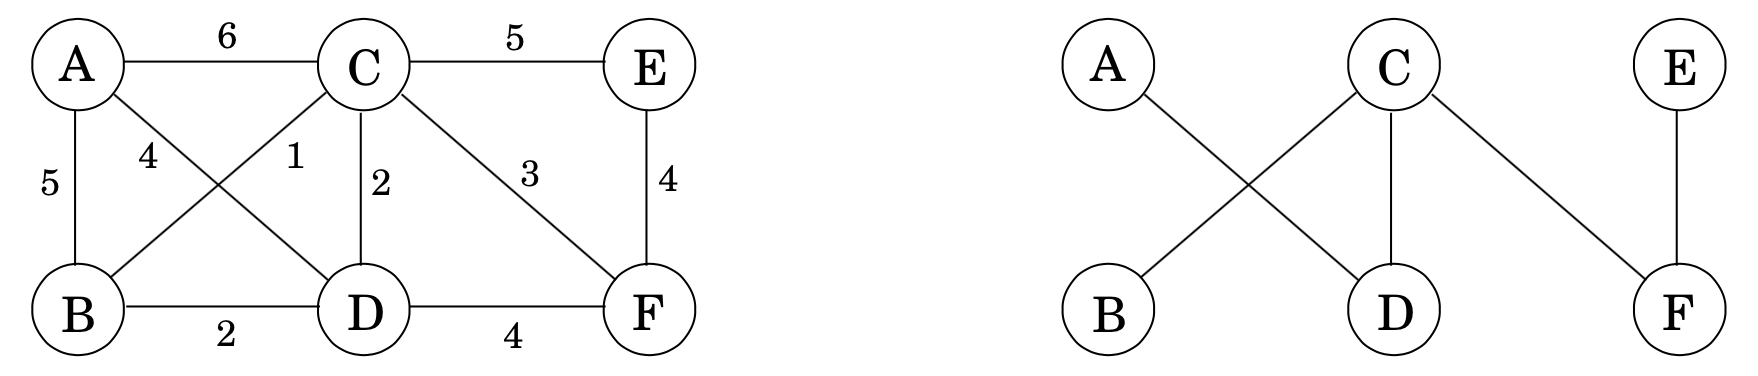
\includegraphics[height=1cm]{images/kruskal-example.png}
% \end{center}

% \subsection*{Properties of Trees (Undirected Acyclic Graphs)}
% \begin{itemize}
%     \item A tree with n nodes has n-1 edges
%     \item Any connected undirected graph G(V,E), with \(|E|=|V|-1\) is a tree
%     \item An undirected graph is a tree if and only if there is a unique path between any pair of nodes.
% \end{itemize}

% \subsubsection*{Cut Property}
% Suppose edges X are part of a minimum spanning tree of \(G=(V,E)\). Pick any subset of nodes S for which X does not cross between S and V-S, and let e be the lightest edge across the partition. Then \(X \cup {e}\) is part of some Minimum Spanning Tree.

% \subsection*{Prim's Algorithm \(O(E\log{E})\)}
% Objective is to also find the MST.
% Alternative to Kruskal's Algorithm; Similar to Dijkstra's)\\
% Standard Data Structure is Priority Queue.
% \textbf{(If Dense: $|E|$ at most $|V^2|$)}\\
% On each iteration, the subtree defined by x grows by one edge, the lightest between a vertex in S and a vertex outside S.

% \begin{verbatim}
% procedure prim(G, w)
% Input: A connected undirected graph G = (V, E) with weights
% Output: A minimum spanning tree defined by the array prev
% for all u in V : 
%     cost(u) = infinity
%     prev(u) = nil
% Pick any initial node $u_0$ 
% cost($u_0$) = 0
% H = makequeue (V) (priority queue with cost-values as keys) 
% while H is not empty:
%     v = deletemin(H) 
%         for each {v, z} in E:
%             if cost(z) > w(v, z): 
%                 cost(z) = w(v, z) 
%                 prev(z) = v 
%                 decreasekey(H, z)
% \end{verbatim}
% \begin{center}
%     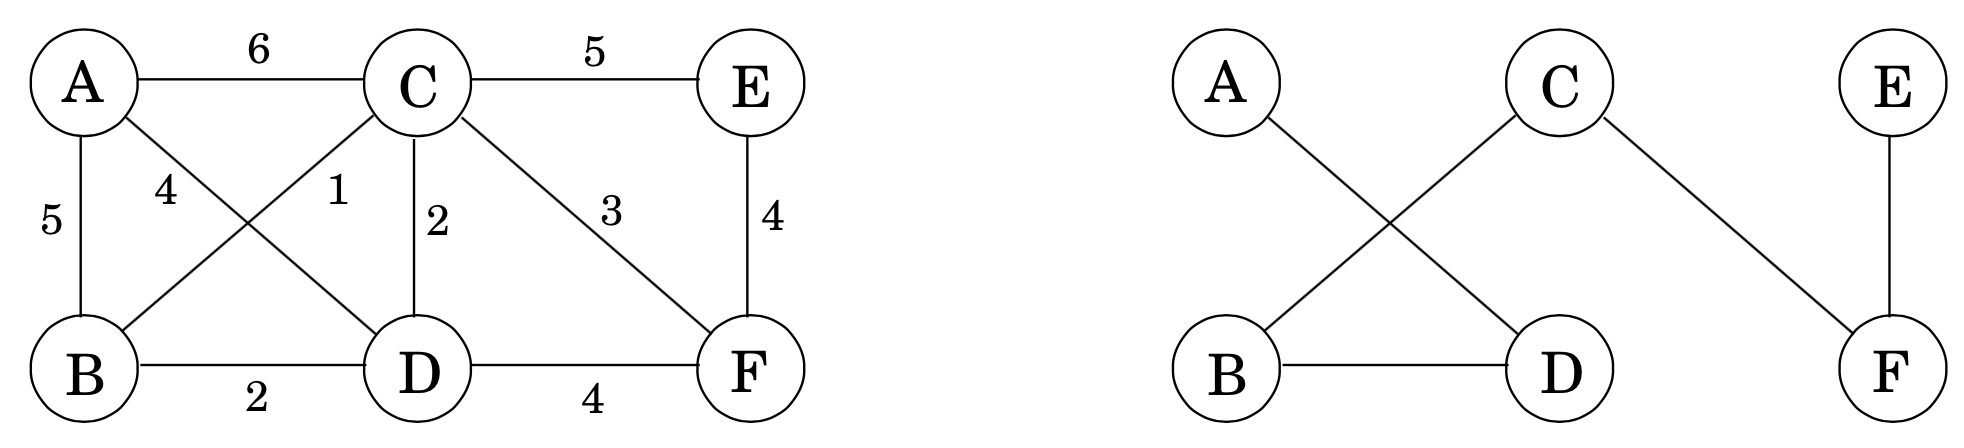
\includegraphics[height=1cm]{images/prims-example.png}
% \end{center}


% \section*{Set Cover Algorithm (Polynomial Time)}
% \begin{verbatim}
% Input: A set of elements B; sets S1,...,Sm
% Output: A selection of the S_i whose union is B.
% Cost: Number of sets picked.

% Repeat until all elements of B are covered:
%     Pick the set Si with the largest number of
%             uncovered elements.
% \end{verbatim}

% \section*{Disjoint Sets Data Structure}
% Contains a function, "find" that returns the root a given set.
% $pi$ refers to the parent node.
% $rank$ refers to the height subtree hanging form that node (number of levels below it).
% \begin{itemize}
% \item For any $x, rank(x) < rank(\pi(x))$.
% \item Any root node of rank $k$ has at least $2^k$ nodes in its tree.
% \item If there are $n$ elements overall, there can be at most $\frac{n}{2^k}$ nodes of rank $k$. The maximum rank is $log n$.
% \end{itemize}
% \begin{verbatim}
% def makeset(x): // O(1)
%     pi(x) = x
%     rank(x) = 0

% def find(x): // O(E log V)
%     while x != pi(x):
%         x=pi(x)
%     return x

% def union(x,y): // O(E log V)
%     if find(x) == find(y):
%         return
%     elif rank(find(x)) > rank(find(y)):
%         pi(find(y)) = find(x)
%     else:
%         pi(find(x))=find(y)
%         if rank(find(x)) == rank(find(y)):
%             rank(find(y)) = rank(find(y)) + 1
% \end{verbatim}

% \section*{Path Compression}
% \begin{verbatim}
% function find(x): 
%     if x != pi(x): pi(x) = find(pi(x)) 
%     return pi(x)
% \end{verbatim}
% Using path compression allows for an amortized cost of O(1) for out Disjoint Set's $union(x, y)$ and $find(x)$ operations.

% \section*{Union Find}
% Uses Disjoint Sets Data Structure\\
% Runs in per operation $Olog*{n}$ which is the number of times you can take a log of n before it becomes 1 or less. It is very slow and for all practical cases is constant. \\
% Basically if find(x) and find(y) return the same value they are in the same graph so do nothing, else add the edge. Then union(x, y).

% Union: Worst case is $O(logN)$ Avg for all Ops is $O(nlog*{n})$ where n is number of elements in Data Structure.

% %%%%%%%%%%%%%%%%%%%%%%%%%%%%%%%%%%%%%%%%%%%%%%%%%
% %%%%%%%%%%%%%%%%%%%%%%%%%%%%%%%%%%%%%%%%%%%%%%%%%
% %%%%%%%%%%%%%%%%%%%%%%%%%%%%%%%%%%%%%%%%%%%%%%%%%
% %%%%%%%%%%%%%%%%%%%%%%%%%%%%%%%%%%%%%%%%%%%%%%%%%
% %%%%%%%%%%%%%%%%%%%%%%%%%%%%%%%%%%%%%%%%%%%%%%%%%

% \section*{Huffman Encoding}
% A means to encode data using the optimal number of bits for each character given a distribution.
% \begin{verbatim}
% func huffman(f):
%     Input: An array f[1...n] of frequencies
%     Output: An encoding tree with n leaves

%     let H be a priority queue of integers, ordered by f
%     for i=1 to n: insert(H,i)
%     for k = n+1 to 2n-1:
%         i=deletemin(H), j=deletemin(H)
%         create a node numbered k with children i,j
%         f[k] = f[i]+f[j]
%         insert(H,k)
% \end{verbatim}

% %%%%%%%%%%%%%%%%%%%%%%%%%

% %\section*{Amortized Analysis}

% %%%%%%%%%%%%%%%%%%%%%%%%%

% \section*{Dynamic Programming}
% Fundamentally DP is carefully bruteforcing the solutions to a problem by turning it into smaller and smaller nested subproblems that remember useful information about its bigger or parent subproblem so that it can eventually reconstruct itself to solve the original problem in a reasonable amount of time. This ``remembrance'' is often done using memoization or parent pointers.\\
% Dynamic Programming has two approaches, which both have the same asymptotic runtime (differ by a constant):
% \begin{enumerate}
% \item \textbf{Top Down:}
% The top down approach uses the recursive idea of breaking the problem into trivially (but still helpful) smaller subproblems and finding a way (through brute force and memorization) to find the maximum or minimum of every permutation what is be left with ever permutation of the subproblems. This is unlike Divide and Conquer which garners its efficiency from reducing its subproblems to massively smaller problems. 
% \item \textbf{Bottom Up:}
% The bottom up approach uses the opposite approach of breaking down the problem into its smallest subproblems and iteratively using the smaller problems to solve bigger and bigger problems until it solves the original problem. A table is often used to keep track of these values. BU is more space efficient than TD, unless you use tail recursion for TD.
% \end{enumerate} 
% You can solve most DP problems by the following steps:
% \begin{enumerate}
% \item Define the subproblems. Know the \# of subproblems. 
% \item Guess a solution for what is not the subproblem (max/min of brute force permutations). Know the \# of guesses.
% \item Relate the subproblems to the parent problem. This is the recursive/iterative step. 
% \item Do the recursion and memoize or iteratively build a table to keep track of previously used values. These can be used to form a DAG. Ensure the DAG for these are acyclic (i.e. have valid topological order or no dependences on parent problems)
% \item Solve the original problem
% ($\theta(\# subproblems * time/subproblem)$)
% \end{enumerate} 
% Choosing Subproblems ($i$ is current problem):
% \begin{itemize}
% \item \textbf{Suffix: } $x[i:] \forall i$ - $O(n)$ (subproblems are broken from i to end)
% Topological Order is right to left. 
% \item \textbf{Prefix: } $x[:i] \forall i$ - $O(n)$ (subproblems are broken from start to i)
% Topological Order is left to right. 
% \item \textbf{Substrings: } $x[i:j] \forall i,j$ - $O(n^2)$ (subproblems are fragments of problem, combination of suffix and prefix)
% Topological Order is increasing substring size. 
% \end{itemize}



% \subsection*{Fibonacci \(O(n)\)}
% \textbf{Recursive:}
% \begin{verbatim}
% memo = {}
% fib(n):
%     if n in memo: return memo[n]
%     if n <= 2: f = 2
%     else: f = fib(n-1) + fib(n-2)
%     memo[n] = f
%     return f
% \end{verbatim}
% \textbf{Iterative:}
% \begin{verbatim}
% fib = []
% fib(n):
%     for k in range(1, n):
%         if k <= 2: f = 2
%         else: f = fib[k-1] + fib[n-2]
%         fib[k] = f
%     return fib[n]
% \end{verbatim}
% \subsection*{Shortest Paths $\theta(VE)$}
% \textbf{For DAGs:}
% For a shortest path (s,v) that uses a limit of, guess take the min of the incoming edge weights into v, say from a node u and then add it to the prefix subproblem of shortest path from (s, u).\\
% \textbf{For General: }
% $S_k (s, v) = $ weight of shortest path from s to v that uses $\le k$ edges.
% $S_k (s, v) = min_{(u, v) in E}(S_{k-1} (s, u) + w(u, v)$\\
% This is Bellman-Ford. 

% \subsection*{Longest Increasing Subsequence: \(O(n^{2})\)}
% Please note that subsequences are any sequences found in another sequences that are not necessarily next to each other (contiguous). Contiguous subsequences are substrings. 
% The following algorithm starts at one side of the list and finds the max length of sequences terminating at that given node, recursively following backlinks. Then given all the lengths of paths terminating at that given node choose the max length. Without memoization, this solution would be exponential time.
% \begin{verbatim}
% L = {}
% for j=1,2,...,n:
%     L[j] = 1+max{L[i]:(i,j) in E}
%     # The (i,j) represents all the edges that go from
%     # a node to j.
% return max(L)
% \end{verbatim}

% \subsection*{Edit Distance (Spelling Suggestions)}
% This algorithm works by basically choosing the min of the options for every given letter. (The 3 options being adding a gap inbetween letters of one of the strings or matching the two letters and moving on.)\\
% ex) Snowy and Sunny have an edit distance of 3 with this configuration
% \begin{verbatim}
% S _ N O W Y
% S U N N _ Y
% \end{verbatim}
% \begin{verbatim}
% for i = 0,1,2,...,m:
%     E(i,0) = i
% for j = 1,2,...,n:
%     E(0,j) = j
% for i = 1,2,...,m:
%     for j = 1,2,...,n:
%         E(i,j) = min{E(i-1,j)+1,E(i,j-1)+1,E(i-1,j-1)
%                     +diff(i,j)}
% return E(m,n)
% \end{verbatim}

% \subsection*{Knapsack \(O(nW)\)}
% Items have a weight and a value, you want to maximize the value within a given weight. (The amount you can carry in your knapsack)\\
% With repetition:
% \[K(\omega)=max_{\texttt{items}}\{K(\omega-\omega_{\texttt{item}})+value\}\]
% Without repetition:
% \[K(\omega,j)=max_{\texttt{available items}}\{K(\omega-\omega_{j},j-1)+V_{j},k(\omega, j-1)\}\]

% \subsection*{Parenthesization \(O(n^3)\)}
% \[C(i,j)=min\{C(i,k)+c(k+1,j)+m_{i-1}\cdot m_{k} \cdot m_{j}\}\]

% \subsection*{Floyd-Warshall \(O(|V|^{3})\)}
% Used for finding shortest paths in a weighted graph with positive or negative edge weights (but with no negative cycles/
% \begin{verbatim}
% for i=1 to n:
%     for j=1 to n:
%         dist(i,j,0) = infinity
%     for all (i,j) in E:
%         dist(i,j,0) = l(i,j)
% for k = 1 to n:
%     for i = 1 to n:
%         for j = 1 to n:
%             dist(i,j,k) = min{dist(i,k,k-1)+
%                               dist(k,j,k-1),
%                               dist(i,j,k-1)}
% \end{verbatim}

% \subsection*{Traveling Salesman Problem (TSP) \(O(n^{2}2^{n})\)}
% Shortest path for visiting all nodes. 
% \begin{verbatim}
% C({1},1)=0
% for s = 2 to n:
%     for all subsets S in {1,2,...,n} of size s and has l:
%         C(S,1) = infinity
%         for all j in S,j != 1:
%             C(S,j) = min{C(S-{j},i)+dij:i in S,i not in j}
% return min over j, C({1,...,n},j)+dj1
% \end{verbatim}

% %%%%%%%%%%%%%%%%%%%%%%%%%

% \section*{Linear Programming}
% Feed into a LP solver like Simplex an \textit{Objective Function} which states if you want to maximize or minimize the equation (max$(x+2y)$), \textit{Constraints} which are limitations for the variables of the Objective Function ($x \ge 0, y \le 600$).
% \begin{enumerate}
%     \item To turn a maximization problem into a minimization (or vice versa) just multiply the coeficients of the objective function by -1.
%     \item To turn an inequality constraint like \(\sum_{i=1}^{n}a_i x_i \leq b\) into an equation, introduce a new variable S and use, \(\sum^n_{i=1}a_{i}x_{i}+s = b\), \(s \geq 0\) (S is known as a slack variable)
%     \item To change an inequality constraint into inequalities rewrite \(ax=b\),\\
%         as \(ax \leq b \texttt{ and } ax \geq b\)
%     \item If a linear program has an unbounded value then its dual must be infeasible.
% \end{enumerate}

% \subsection*{Simplex}
% Typically Polynomial time; Worst Case Exponential.
% \begin{verbatim}
% let v be any vertex of the feasible region
% while there is a neighbor v' of v with a better value:
%     set v = v'
% return v
% \end{verbatim}


% \subsection*{Max Flow}
% Construct graph G that is a simple directed graph with source s and sink t. No negative capacities are possible.\\
% Construct a Residual Graph with forward edges for the amount of capacity that is not being used (capacity - current use) and a back edge for what is currently being used. 

% \subsubsection*{Ford-Fulkerson}
% Start with no flow on your graph. Find a path using DFS. Then create a residual graph. We can now use DFS for finding a path from s to t in the residual graph. If one exists we are not optimally using our flow. We then find the edge with the LEAST capacity edge - this is our bottleneck - and add flow onto all the edges in that path up to the capacity that is not being used by the bottleneck edge, hereby maximizing the flow of the path. Our new flow is guaranteed to be better. Create a new residual graph and repeat until no path in the residual graph can be found from s to t. This will happen when capacity = current use, as we lose our forward edge and only have a back edge.\\
% This algorithm will sometimes decrease flow in one area to increase flow in another. Max flow is the total weights of incoming edges to the sink. Runtime would be $O(E * M)$, where $M$ is the number of iterations and $E$ is the time to find a path. This can also be stated as $O($maxflow$*E)$. However this may not terminate. If you use BFS instead of DFS you are using the Edmonds-Karp Algorithm which will terminate and has complexity $O(V*(E)^2)$, which is better for large networks.
% \begin{center}
% 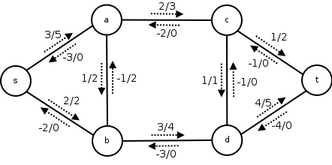
\includegraphics[scale=.25]{images/flow.png}
% 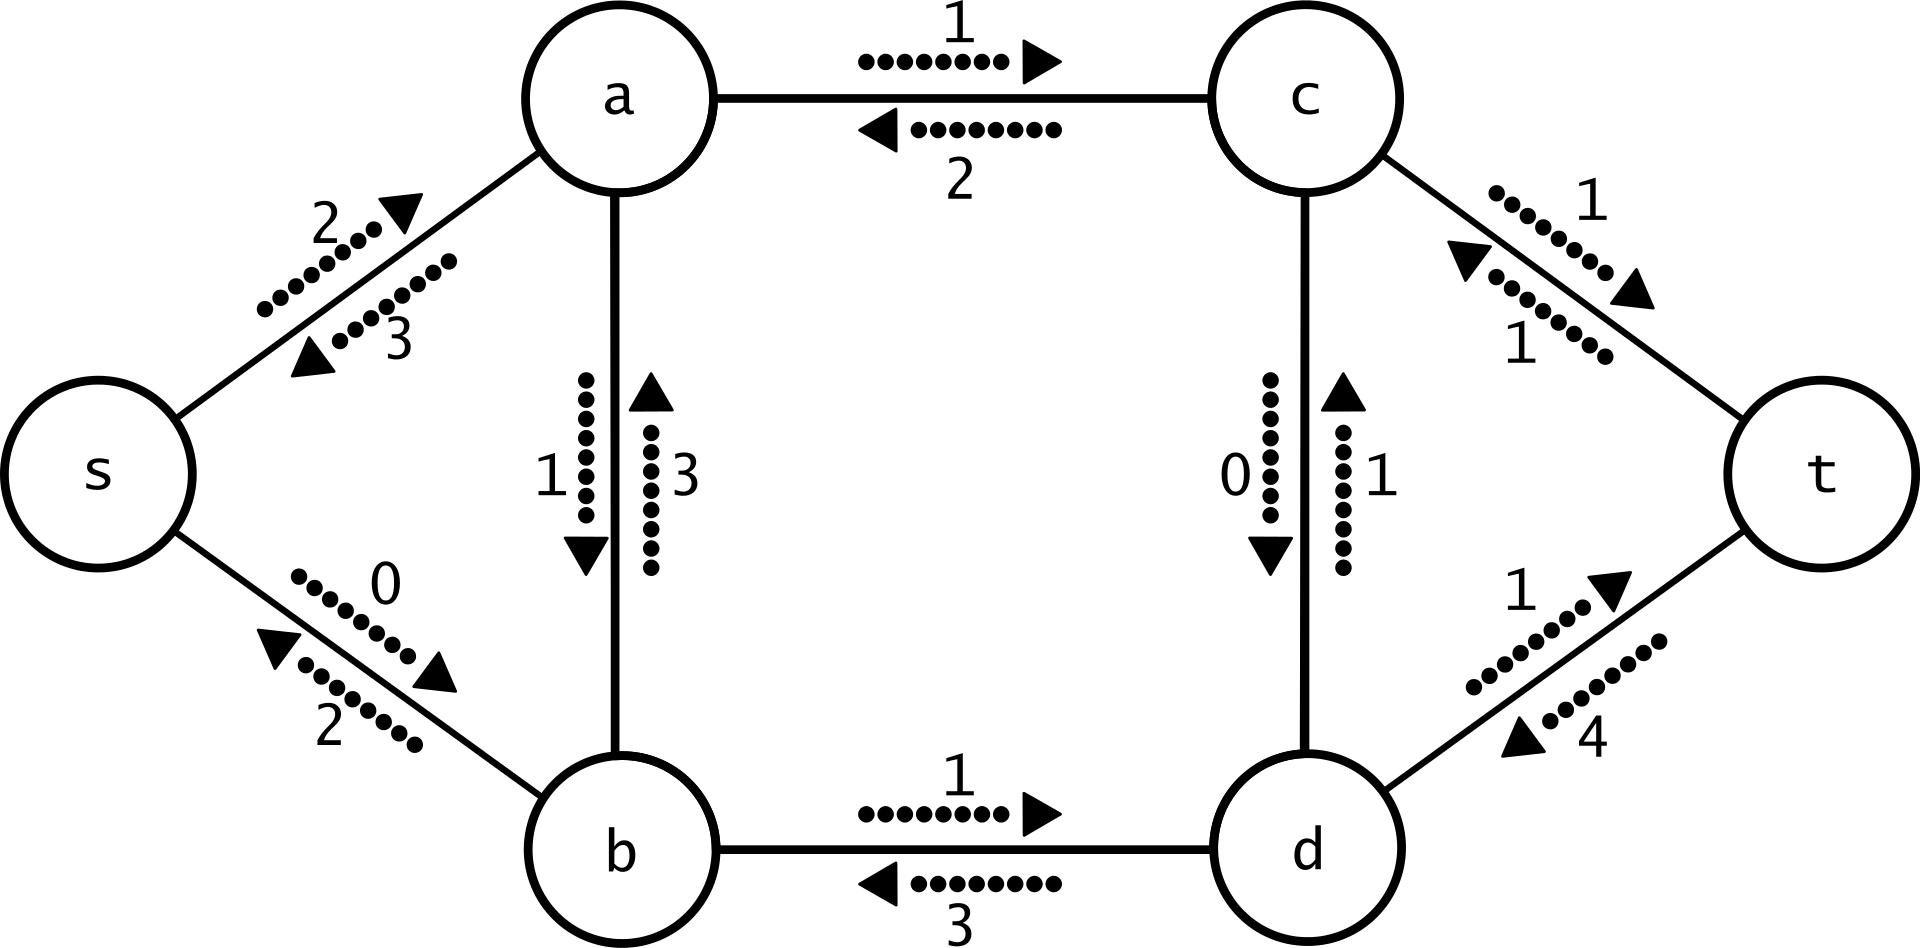
\includegraphics[scale=.06]{images/residual.png}
% \end{center}

% \subsubsection*{Max Flow Min Cut Theorem}
% The size of the maximum flow in a network equals the capacity of the smallest (s,t)-cut, where and (s,t)-cut partitions the vertices into two disjoint groups L and R such that s (start) is in L and t (goal) is in R.

% \subsubsection*{Bipartite Matching}
% Explained by Example: list of boys, list of girls, if boy likes girl, a direct edge exists from boy to girl. Is there a perfect matching?
% Create source node $s$ and sink node $t$, $s$ has outgoing edges to all the boys, and $t$ has incoming edges from all the girls. Give every edge a capacity of one (obviously). A flow exists if there is a flow into $t$ with size equal to number of couples. 

% %%%%%%%%%%%%%%%%%%%%%%%%%

% \section*{Computational Complexity}
% We use Computational Complexity to determine classifications for our algorithms to know if they are feasible. 

% \subsection*{Decision vs. Search Problems}
% \textbf{Decision Problem: }Computational problem that answers ``Yes'' or ``No''. Our input can be any possible string (binary, ASCII), and it will answer either 0 or 1 depending upon weather the solution is correct or not. This type of problem determines our classes.\\
% \textbf{Search Problem: }Computational problem tasked with not if a solution exists, but what one is. Decision problems can be derived from Search problems which are generally always more difficult. 

% \subsection*{Classifications}
% \begin{itemize}
% \item \textbf{P}: The set of all search problems that are solvable in a reasonable amount of time (Polynomial time).
% \item \textbf{NP (Nondeterministic Polynomial)}: The set of all search problems whose solution can be checked in Polynomial time (includes P) - there might exist search problems whose solutions can not be checked in Polynomial time. A solution may not necessary be found in a reasonable amount of time ($2^n$ and $n!$ algorithms can be in NP). Called NP because if you had the power to guess correct every time it would work in Polynomial time, making it non-deterministic. Should be called ``Guessing in P''.
% \item \textbf{NP-Hard:} Any problem in NP can be reduced to this problem in Polynomial time, so it is at least as difficult or ``hard'' as any NP problem. The Halting Problem is NP hard and also impossible to solve in a finite amount of time, so this idea is not always practically useful for reductions. Most NP-Hard problem are NOT in NP, but those that are, are NP-Complete.
% \item \textbf{NP-Complete: }Problem that is not only as hard as every problem in NP, but is also in NP. (NP-Hard and in NP). Any NP problem can be reduced to one of these in Polynomial time. It is often useful to prove the difficulty of problems. These are the hardest problems in NP and the reason why P = NP can revolutionize things. 
% \end{itemize}
% \begin{center}
% 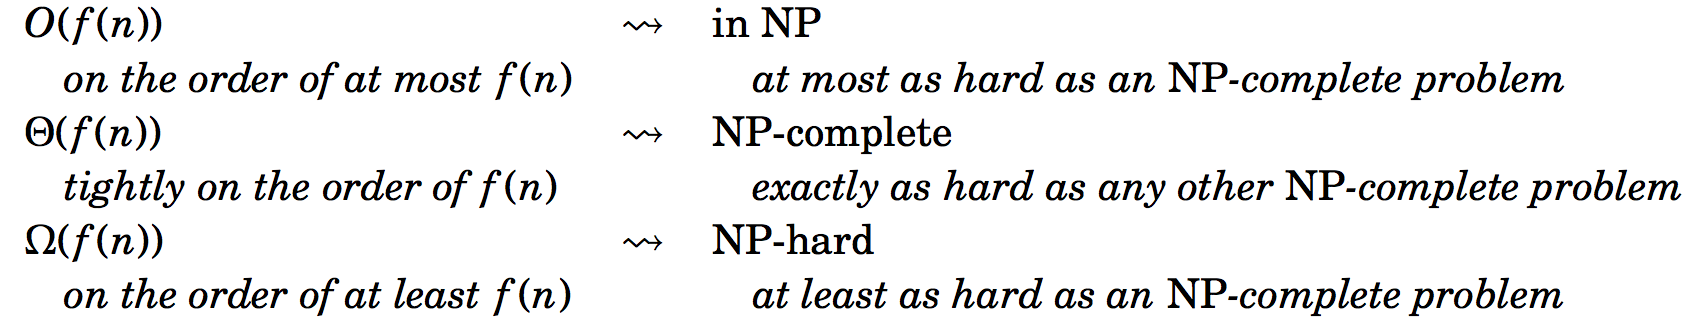
\includegraphics[scale=.25]{images/analogy.png}
% \end{center}

% \subsection*{Common NP-Complete Problems}
% \begin{center}
% \begin{tabular}{|c|c|}
%     \hline
%     Hard problems(NP-complete) & Easy problems (in P)\\
%     \hline
%     \hline
%     3SAT & 2SAT, HORN SAT\\
%     Traveling Salesman Problem & Minimum Spanning Tree\\
%     Longest Path & Shortest Path\\
%     3D Matching & Bipartite Matching\\
%     Knapsack & Unary Knapsack\\
%     Independent Set & Independent Set on trees\\
%     Integer Linear Programming & Linear Programming\\
%     Rudrata Path & Euler Path\\
%     Balanced Cut & Minimum Cut\\
%     \hline
% \end{tabular}
% \end{center}

% \subsubsection*{Satisfiability (SAT)}
% This is the prototypical NP-Complete problem that everything started from.
% Say you have some Boolean expressions written using only AND, OR, NOT, variables, and parentheses (Example: $x_1 \land x_2 \lor x_3$). The SAT problem is given any one of these expressions, is there some assignment of TRUE and FALSE values to the variables that will make the entire expression TRUE? 
% \subsubsection*{3SAT}
% This is a stricter version of the SAT problem in which the statement is divided into clauses where each clause can have exactly 3 literals. (Example: $(x_1 \lor x_2 \lor x_3)\land(x_4 \lor x_5 \lor x_6)$). For these you want to find whether there exists values for $x_1 ... x_6$such that the boolean evaluates to TRUE.
% \subsubsection*{CircuitSAT}
% Given a circuit of logic gates with a single output and no loops find there a setting of the inputs that causes the circuit to output 1.
% \subsubsection*{Integer Linear Programming} 
% Solve a problem using linear objective function and linear inequalities, WHILE constraining the values of the variables to integers. 
% \subsubsection*{Traveling Salesman Problem (TSP)}
% Find the \textit{shortest path} in a graph that visits all the vertices exactly once before returning home. This comes from the idea of a traveling salesman wanting to efficiently visit all the cities to sell his wares. 
% \subsubsection*{Rudrata/Hamiltonian Cycle}
% Given a graph find if there a cycle that passes through each vertex exactly once, or report one doesn't exist. 
% \subsubsection*{Rudrata/Hamiltonian Path}
% Given a path starting at $s$ and ending at $t$ that goes through each vertex exactly once.
% \subsubsection*{Independent Set}
% Given a graph and a number $g$, the aim is to find $g$ vertices that are independent meaning that no two of which have share an edge. 
% \subsubsection*{Graph 3-Coloring}
% Given an undirected graph G = (V,E) find a valid 3-coloring C such that no two vertices sharing the same edge have the same color, or report that such an ordering doesn't exist. 


% %%%%%%%%%%%%%%%%%%%%%%%%%

% \section*{Reductions}
% Reductions are an incredible useful tool for either turning a search problem we don't know how to solve into one we do, or proving that a search problem can not be solved or is hard to solve by reducing it to problem that is one of those two things.\\
% - We know how to solve $B$ in a reasonable amount of time and we want to use this knowledge to solve $A$.\\
% - We denote a reduction from $A$ to $B$ as $A \to B$. Difficultly flows in the direction of the arrow.\\
% - If we can reduce our unknown problem $A$ into a known problem $B$ then $B$ must be as hard if not even harder to solve than $A$. A way to mathematically write this is $A \le_{p} B$. $A$ thereby provides a lower bound of hardness for $B$.\\ 
% - Reduction can be composed as well: if you can reduce $A \to B$ and $B \to C$ then $A \to C$.\\
% - Any search problem in NP can be reduced to an NP-Hard Problem in Polynomial Time but this is not always useful (like Halting Problem) \\
% - Any search problem in NP can also be reduced to an NP-Complete Problem in Polynomial Time.\\
% - Any problem that is NP-Complete is reducible to any other problem that is also NP-Complete which is very useful.
% \subsubsection*{Reduction Tree}
% 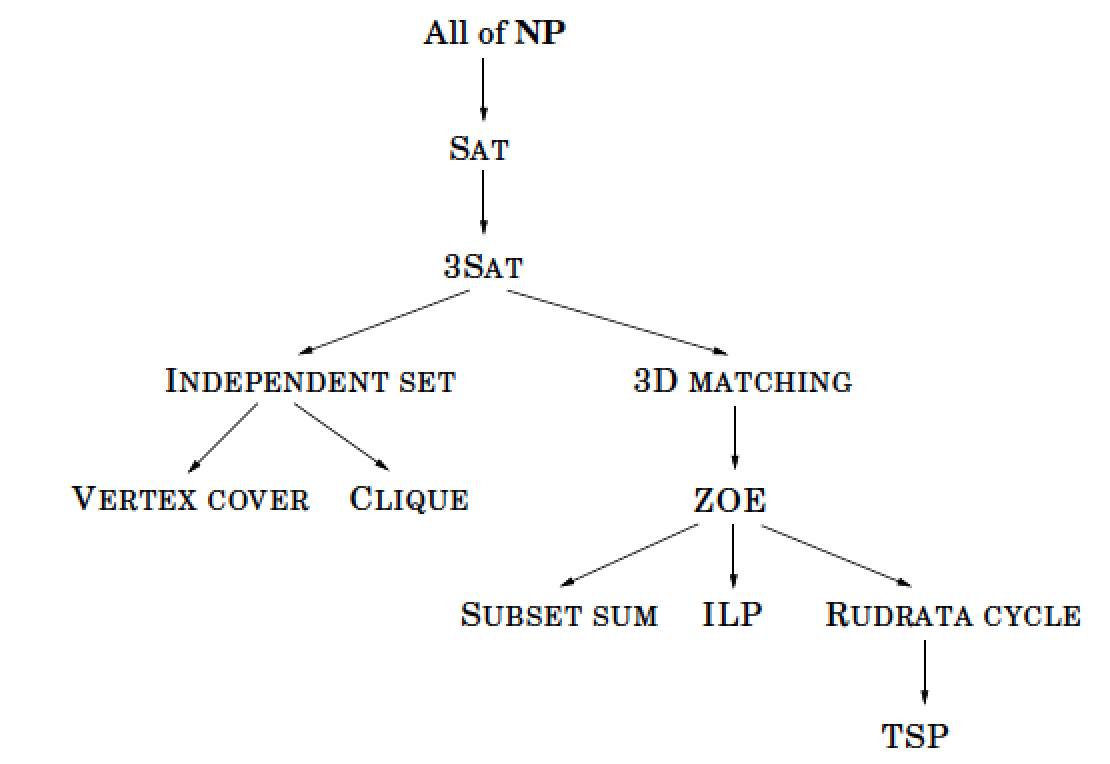
\includegraphics[scale=.4]{images/reductions.png}


% %%%%%%%%%%%%%%%%%%%%%%%%%
% \subsection*{Dealing with NP-Completeness}

% \subsubsection*{Backtracking}
% Backtracking is the idea of rejecting a portion of a solution that in some manner proves to be useless without fully processing it. Say if you find a violation of a certain criteria set in your algorithm, then you can stop, no longer process the children of that node and move up to another node to try its luck. It's not going to work anyways since it didn't work for the parent. \\
% More abstractly, a backtracking algorithm requires a test that looks at a subproblem and quickly declares one of three outcomes:

% \begin{itemize}
% \item Failure: the subproblem has no solution. backtrack.
% \item Success: a solution to the subproblem is found. 
% \item Uncertainty: branch again and retry.
% \end{itemize}

% \begin{verbatim}
% Start with some problem P0
% Let S = {$P_0$}, the set of active subproblems 
% Repeat while S is nonempty:
%   choose a subproblem P ∈ S and remove it from S 
%   expand it into smaller subproblems P_1, P_2, . . . , P_k 
%   For each P_i:
%     If test (P_i) succeeds: 
%         halt and announce this solution
%     If test (P_i) fails: 
%         discard Pi Otherwise: add P_i to S
% Announce that there is no solution
% \end{verbatim}


% \subsubsection*{Branch-and-bound}
% Another technique in which you don't process off a whole portion of a tree because due to some formula you know it will not offer a more efficient solution. 
% For example if you need to choose find a Hamiltonian path and you have thus far a path $A$ with weight 3 and another path $B$ with weight 7, given the information that the MST for the rest of the nodes for each path is of length 12, you can disregard the brute force calculation of the longer path, since it won't be better than what you already have.\\
% Finding the lowerbound is the really tricky part. 
% \begin{verbatim}
% Start with some problem P0
% Let S = {P0}, the set of active subproblems 
% bestsofar = infinity 
% Repeat while S is nonempty:
% 	choose a subproblem (partial solution) 
% 	P in S and remove it from S 
% 	expand it into smaller subproblems P_1, P_2, ..., P_k
% 	For each P_i:
% 		If P_i is a complete solution: update bestsofar
% 		else if lowerbound(Pi) < bestsofar: add Pi to S 
%     return bestsofar
% \end{verbatim}
% %%%%%%%%%%%%%%%%%%%%%%%%%

% \subsubsection*{Approximation Ratio}

% Finding the OPT(I) is the challenging part, but it is always positive. 

% For Minimization:
% $\alpha_{A} = max (I)$ of $\frac{A(I)}{OPT(I)}$

% For Maximization:
% $\alpha_{A} = max (I)$ of $\frac{OPT(I)}{A(I)}$

% Vertex Cover
% Input: An undirected graph G = (V, E).
% Output: A subset of the vertices S contained in V that touches every edge. Goal: Minimize |S|.

% Special Case of Set Cover, works in $\O (log n)$


% %%%%%%%%%%%%%%%%%%%%%%%%%

% \section*{Machine Learning Algorithms}

% Use big data set to train a classifier, which can then categorize new data.
% Data partitions: take $80\%$ of data and use it as training, ie, feed into classifier both the data and expected result. use 20% for validation to get error rate and see how well you are performing.

% Data is encoded as “features”, which is usually a vector of numbers, often normalized to floats between 0.0 and 1.0, These features are used to train the classifier.

% \subsection*{K Nearest Neighbors}
% We are working in a multidimensional space, with a dimension for each feature index. We then take all of our points and store them in some data structure that allows us to query for the nearest neighbors to an arbitrary point. The way the classification works is given a new point, we plot it, and get the K nearest neighbors to it. (Those neighbors are the test points we used to train the classifier.) Once we get those neighbors, we take a majority vote on their labels and figure out what this new unseen point actually is.\\

% A small example: Imagine you are applying to a credit card. They ask for you age, income, and number of credit cards. From this, they create a 3 dimensional feature: {age, income, count}. The company takes your data and checks their classifier. The classifier plots your point and sees that you fall right in the middle of a cluster of people who always pay their bills on time. You are then judged as a good client.

% This is our classify algorithm: \\
% Runs in $\theta(nd)$
% \begin{verbatim}
% def Classify(x):
%   set i* = 1
%   for i - 2, 3,..., n:
%     if ||x-x_i|| < ||x-x_i*||, set i* = i
%   return y_i*
% \end{verbatim}

% Now to make this more accurate by using a voting system:\\

% Given x, we compute the distance from x to each observation in the training set, and then keep the k
% closest observations. Intuitively, the class of each of them gives a plausible suggestion for the class
% of x. Therefore, we can treat each as a vote for the class of x. We take these k votes, find which
% class received the most votes, and classify x with this class. In many applications, this improves
% the accuracy of the nearest neighbor classifier by “smoothing” out the classifier’s predictions.\\

% For boolean classification, it is often convenient to choose
% k to be odd, to avoid ties.\\

% Runs in $\theta(n(d + lg k))$ but for small values of k this is almost as fast as the classifier. 


%%%%%%%%%%%%%%%%%%%%%%%%%


%\rule{0.3\linewidth}{0.1pt}
\scriptsize

\end{multicols}
\end{document}
